% =====================================================================
%  PULSE --- two-page high-level architecture
%  Compile:  pdflatex pulse-overview.tex
% =====================================================================
\documentclass[10pt,a4paper]{article}
\usepackage[utf8]{inputenc}
\usepackage[T1]{fontenc}
\usepackage{lmodern}
\usepackage{microtype}
\usepackage[margin=1.4cm,top=1.3cm,bottom=1.2cm]{geometry}
\usepackage{xcolor}
\usepackage{booktabs}
\usepackage{array}
\usepackage{enumitem}
\usepackage{graphicx}
\usepackage{tikz}
\usetikzlibrary{arrows.meta,positioning,fit,backgrounds,calc}
\usepackage[hidelinks]{hyperref}
\DeclareUnicodeCharacter{20B9}{Rs.}

\definecolor{ink}{HTML}{16202C}
\definecolor{slate}{HTML}{4A5768}
\definecolor{mist}{HTML}{E8ECF1}
\definecolor{paper}{HTML}{F7F9FB}
\definecolor{navy}{HTML}{1D3B63}
\definecolor{teal}{HTML}{0E7C7B}
\definecolor{amber}{HTML}{B8860B}
\definecolor{brick}{HTML}{9B2C2C}
\definecolor{moss}{HTML}{3F6C3F}
\definecolor{plum}{HTML}{6B3FA0}

\pagestyle{empty}
\setlength{\parindent}{0pt}
\setlength{\parskip}{3pt}

\newcommand{\code}[1]{\texttt{\small #1}}
\newcommand{\rs}[1]{Rs.\,#1}
\newcommand{\hd}[1]{\vspace{4pt}{\color{navy}\large\bfseries #1}\par\vspace{2pt}}
\newcommand{\shd}[1]{{\color{slate}\bfseries\footnotesize #1}\par\vspace{1pt}}

\tikzset{
  box/.style={rectangle, rounded corners=2pt, draw=slate, fill=white, line width=0.6pt,
              align=center, inner sep=4pt, font=\scriptsize},
  modelbox/.style={box, draw=plum, fill=plum!7, font=\scriptsize\bfseries},
  detbox/.style={box, draw=teal, fill=teal!7},
  guardbox/.style={box, draw=brick, fill=brick!7},
  databox/.style={box, draw=navy, fill=navy!7},
  lbl/.style={font=\tiny\itshape, text=slate, align=center},
  flow/.style={-{Stealth[length=4pt]}, draw=slate, line width=0.6pt},
  backflow/.style={-{Stealth[length=4pt]}, draw=amber, line width=0.6pt, dashed},
}

\newsavebox{\fitbox}
\newenvironment{fitpic}
  {\par\vspace{3pt}\begin{center}\begin{lrbox}{\fitbox}}
  {\end{lrbox}%
   \ifdim\wd\fitbox>\textwidth \resizebox{\textwidth}{!}{\usebox{\fitbox}}%
   \else \usebox{\fitbox}\fi
   \end{center}\vspace{2pt}}

\begin{document}

% =====================================================================
% PAGE 1
% =====================================================================
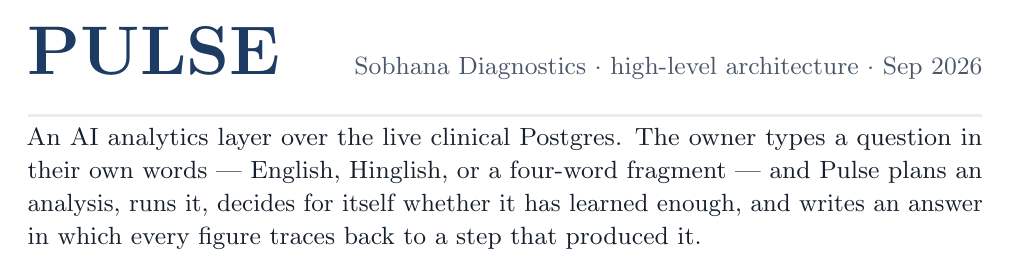
\begin{tikzpicture}[remember picture]
\node[inner sep=0pt] (t) {%
\begin{minipage}{\textwidth}
{\color{navy}\Huge\bfseries PULSE}\hfill{\color{slate}\small Sobhana Diagnostics $\cdot$ high-level architecture $\cdot$ Sep 2026}\\[2pt]
{\color{mist}\hrule height 1.2pt}\vspace{4pt}
{\color{ink}\small An AI analytics layer over the live clinical Postgres. The owner types a question in
their own words --- English, Hinglish, or a four-word fragment --- and Pulse plans an analysis, runs
it, decides for itself whether it has learned enough, and writes an answer in which every figure
traces back to a step that produced it.}
\end{minipage}};
\end{tikzpicture}

\vspace{2pt}
\hd{How one question flows}
\vspace{-4pt}

\begin{fitpic}
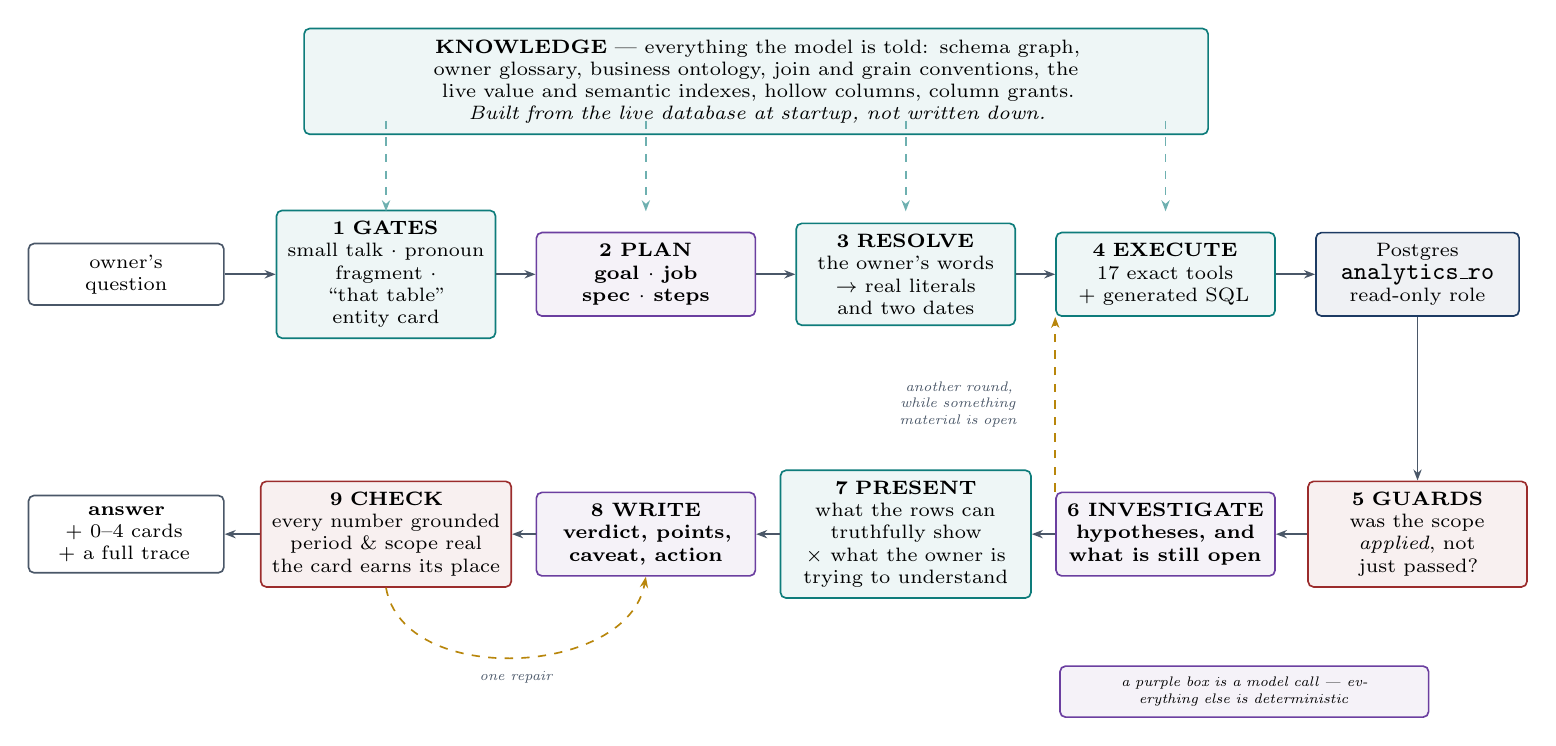
\begin{tikzpicture}[x=1cm,y=1cm, every node/.style={font=\scriptsize}]

\node[detbox, text width=112mm] at (8.0,2.45)
  {\textbf{KNOWLEDGE} --- everything the model is told: schema graph, owner glossary, business ontology,
   join and grain conventions, the live value and semantic indexes, hollow columns, column grants.\\
   \scriptsize\itshape Built from the live database at startup, not written down.};

\node[box,      text width=22mm] (q)    at (0.0,  0) {owner's\\question};
\node[detbox,   text width=25mm] (gate) at (3.3,  0) {\textbf{1 GATES}\\small talk $\cdot$ pronoun\\fragment $\cdot$ ``that table''\\entity card};
\node[modelbox, text width=25mm] (plan) at (6.6,  0) {\textbf{2 PLAN}\\goal $\cdot$ job\\spec $\cdot$ steps};
\node[detbox,   text width=25mm] (res)  at (9.9,  0) {\textbf{3 RESOLVE}\\the owner's words\\$\to$ real literals\\and two dates};
\node[detbox,   text width=25mm] (exe)  at (13.2, 0) {\textbf{4 EXECUTE}\\17 exact tools\\$+$ generated SQL};
\node[databox,  text width=23mm] (db)   at (16.4, 0) {Postgres\\\code{analytics\_ro}\\read-only role};

\node[guardbox, text width=25mm] (grd)  at (16.4,-3.3) {\textbf{5 GUARDS}\\was the scope\\\emph{applied}, not\\just passed?};
\node[modelbox, text width=25mm] (inv)  at (13.2,-3.3) {\textbf{6 INVESTIGATE}\\hypotheses, and\\what is still open};
\node[detbox,   text width=29mm] (cap)  at (9.9, -3.3) {\textbf{7 PRESENT}\\what the rows can truthfully show\\$\times$ what the owner is\\trying to understand};
\node[modelbox, text width=25mm] (wr)   at (6.6, -3.3) {\textbf{8 WRITE}\\verdict, points,\\caveat, action};
\node[guardbox, text width=29mm] (chk)  at (3.3, -3.3) {\textbf{9 CHECK}\\every number grounded\\period \& scope real\\the card earns its place};
\node[box,      text width=22mm] (out)  at (0.0, -3.3) {\textbf{answer}\\$+$ 0--4 cards\\$+$ a full trace};

\foreach \x in {3.3,6.6,9.9,13.2} \draw[flow, dashed, draw=teal!60] (\x,1.95) -- (\x,0.80);

\draw[flow](q)--(gate); \draw[flow](gate)--(plan); \draw[flow](plan)--(res);
\draw[flow](res)--(exe); \draw[flow](exe)--(db);
\draw[flow](db)--(grd);
\draw[flow](grd)--(inv); \draw[flow](inv)--(cap); \draw[flow](cap)--(wr);
\draw[flow](wr)--(chk); \draw[flow](chk)--(out);

\draw[backflow] (inv.north west) -- node[lbl,left=0.5mm,text width=21mm]{another round, while something material is open} (exe.south west);
\draw[backflow] (chk.south) to[out=280,in=260] node[lbl,below=0.5mm]{one repair} (wr.south);

\node[modelbox, text width=44mm, font=\tiny\itshape] at (14.2,-5.3)
  {a purple box is a model call --- everything else is deterministic};
\end{tikzpicture}
\end{fitpic}

\vspace{-2pt}
{\footnotesize\color{slate}\textbf{Cost of that:} 3 model calls and 4--6 seconds for a figure. A real
investigation is a median of 7 calls and 22--32 seconds, with a hard ceiling of 180s that the answer
must \emph{disclose} if it hits.}

\vspace{6pt}
\hd{What each layer is responsible for}
\vspace{-6pt}

{\footnotesize
\begin{tabular}{@{}p{2.1cm}p{5.6cm}p{10.2cm}@{}}
\toprule
\textbf{Layer} & \textbf{Decides} & \textbf{The rule it exists to enforce}\\
\midrule
\textbf{Gates} & is this even an analysis question & ``In that table'' is a \emph{conversation} problem, not an
 entity lookup. A pronoun with nothing to point at is a question, not a search.\\
\textbf{Knowledge} & everything the model is told & Built from the live database at startup, not written down. The
 \emph{only} lever measured to move accuracy on this workload.\\
\textbf{Plan} & goal, analytical job, scope, period, steps & The analyst writes a \emph{contract} before any SQL
 exists --- the owner's word next to the resolved literal.\\
\textbf{Resolve} & what the owner's words mean here & Resolved against the owner's own sentence, never the
 planner's paraphrase. ``CT'' is a modality here, not the lab code for Clotting Time.\\
\textbf{Execute} & 17 exact tools, or generated SQL & A registry tool is free and repeatable; \code{query} is
 general. A close number is a wrong number, so a qualifier the tools cannot express goes to \code{query}.\\
\textbf{Guards} & may this figure be used at all & A tool that applied a scope \emph{says so}. Silence is a refusal ---
 a wrong number with a confident label is the worst thing this system can do.\\
\textbf{Investigate} & is anything material still open & Continuing is a consequence of an unresolved claim, not of
 the model's appetite. Stopping always has a stated reason.\\
\textbf{Present} & what may be drawn, and how much goes in prose & The \emph{rows} decide what a card can
 truthfully show; the \emph{job} decides which of those is useful. No words are matched against the question.\\
\textbf{Check} & may this answer ship & Every figure must come from a step or follow from two that do. An
 unclosed investigation must say so in the verdict, not a trailing caveat.\\
\bottomrule
\end{tabular}}

\vfill
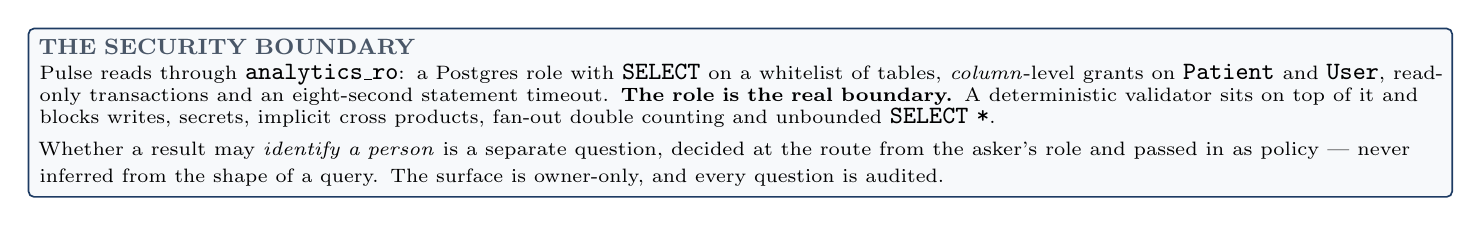
\begin{tikzpicture}
\node[box, draw=navy, fill=paper, text width=178mm, align=left, font=\footnotesize]
 {\shd{THE SECURITY BOUNDARY}
  \scriptsize
  Pulse reads through \code{analytics\_ro}: a Postgres role with \code{SELECT} on a whitelist of tables,
  \emph{column}-level grants on \code{Patient} and \code{User}, read-only transactions and an eight-second
  statement timeout. \textbf{The role is the real boundary.} A deterministic validator sits on top of it and
  blocks writes, secrets, implicit cross products, fan-out double counting and unbounded \code{SELECT *}.\\[2pt]
  Whether a result may \emph{identify a person} is a separate question, decided at the route from the asker's
  role and passed in as policy --- never inferred from the shape of a query. The surface is owner-only, and
  every question is audited.};
\end{tikzpicture}

\clearpage

% =====================================================================
% PAGE 2
% =====================================================================
{\color{navy}\Large\bfseries Why it is built this way}\hfill{\color{slate}\small page 2 of 2}\\[2pt]
{\color{mist}\hrule height 1.2pt}

\vspace{4pt}
{\footnotesize Sixteen days, eleven architectures, roughly 9{,}000 measured model calls. Two results
did all the shaping.}

\vspace{4pt}
\begin{fitpic}
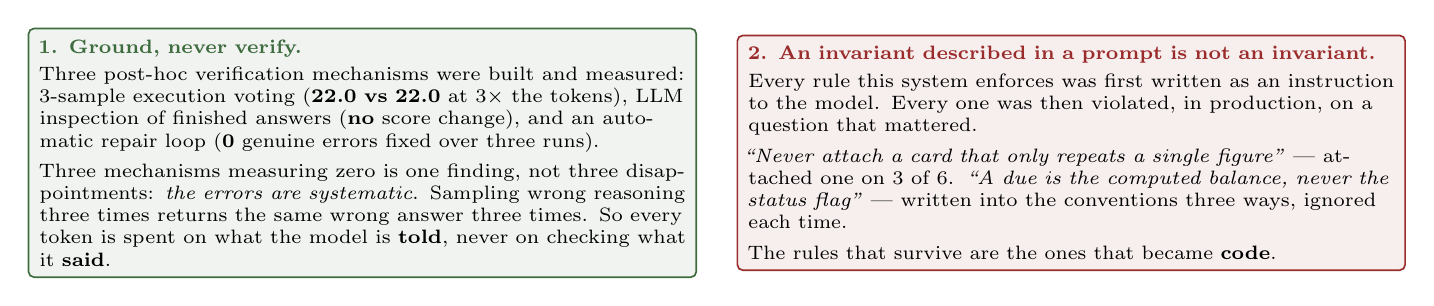
\begin{tikzpicture}[every node/.style={font=\scriptsize}]
\node[box, draw=moss, fill=moss!8, text width=82mm, align=left] (a)
 {\textbf{\color{moss}1. Ground, never verify.}\\[2pt]
  Three post-hoc verification mechanisms were built and measured:
  3-sample execution voting (\textbf{22.0 vs 22.0} at 3$\times$ the tokens), LLM inspection of finished
  answers (\textbf{no} score change), and an automatic repair loop (\textbf{0} genuine errors fixed over
  three runs).\\[3pt]
  Three mechanisms measuring zero is one finding, not three disappointments: \emph{the errors are
  systematic}. Sampling wrong reasoning three times returns the same wrong answer three times.
  So every token is spent on what the model is \textbf{told}, never on checking what it \textbf{said}.};
\node[box, draw=brick, fill=brick!8, text width=82mm, align=left, right=5mm of a] (b)
 {\textbf{\color{brick}2. An invariant described in a prompt is not an invariant.}\\[2pt]
  Every rule this system enforces was first written as an instruction to the model. Every one was
  then violated, in production, on a question that mattered.\\[3pt]
  \emph{``Never attach a card that only repeats a single figure''} --- attached one on 3 of 6.
  \emph{``A due is the computed balance, never the status flag''} --- written into the conventions
  three ways, ignored each time.\\[3pt]
  The rules that survive are the ones that became \textbf{code}.};
\end{tikzpicture}
\end{fitpic}

\vspace{12pt}
\hd{The two execution paths, and the wall between evidence and the owner}
\vspace{-4pt}

\begin{fitpic}
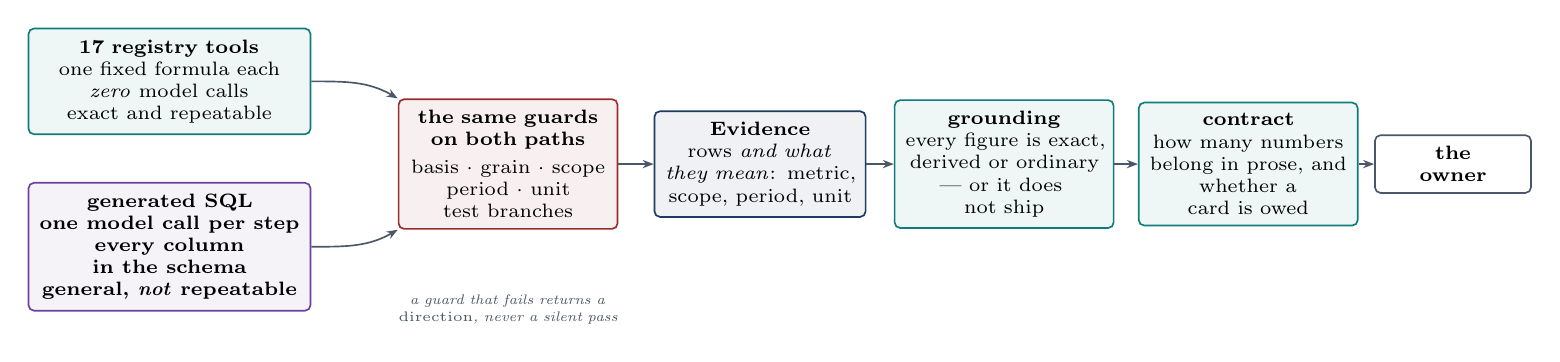
\begin{tikzpicture}[x=1cm,y=1cm, every node/.style={font=\scriptsize}]
\node[detbox,   text width=33mm] (reg) at (0.0, 1.05) {\textbf{17 registry tools}\\one fixed formula each\\\emph{zero} model calls\\exact and repeatable};
\node[modelbox, text width=33mm] (gen) at (0.0,-1.05) {\textbf{generated SQL}\\one model call per step\\every column in the schema\\general, \emph{not} repeatable};
\node[guardbox, text width=25mm] (g1)  at (4.3, 0)    {\textbf{the same guards}\\\textbf{on both paths}\\[2pt] basis $\cdot$ grain $\cdot$ scope\\period $\cdot$ unit\\test branches};
\node[databox,  text width=24mm] (ev)  at (7.5, 0)    {\textbf{Evidence}\\rows \emph{and what}\\\emph{they mean}: metric,\\scope, period, unit};
\node[detbox,   text width=25mm] (gr)  at (10.6, 0)   {\textbf{grounding}\\every figure is exact,\\derived or ordinary\\--- or it does not ship};
\node[detbox,   text width=25mm] (con) at (13.7, 0)   {\textbf{contract}\\how many numbers\\belong in prose, and\\whether a card is owed};
\node[box,      text width=17mm] (own) at (16.3, 0)   {\textbf{the}\\\textbf{owner}};
\draw[flow] (reg.east) to[out=0,in=150] (g1.north west);
\draw[flow] (gen.east) to[out=0,in=210] (g1.south west);
\draw[flow](g1)--(ev); \draw[flow](ev)--(gr); \draw[flow](gr)--(con); \draw[flow](con)--(own);
\node[lbl, text width=30mm] at (4.3,-1.85) {a guard that fails returns a \emph{direction}, never a silent pass};
\end{tikzpicture}
\end{fitpic}

\vspace{2pt}
{\footnotesize\color{slate}Seventeen tools are deterministic and free, so a plan can look at six things
before deciding what matters. Only \code{query} buys latency --- and only \code{query} can give two
different answers to the same question, which is why the guards sit on both paths and not just on it.}

\vfill
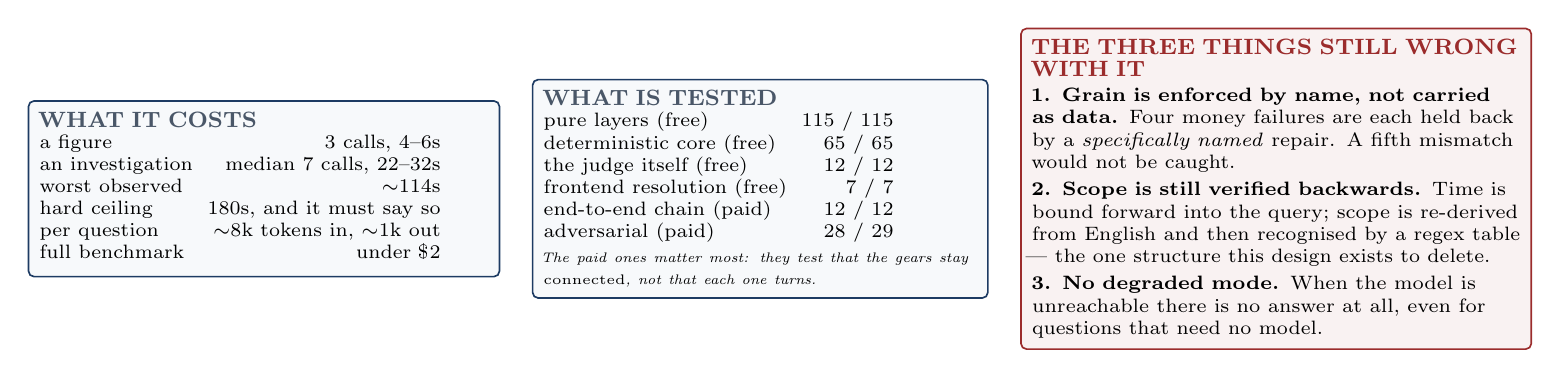
\begin{tikzpicture}[every node/.style={font=\footnotesize}]
\node[box, draw=navy, fill=paper, text width=57mm, align=left] (n1)
 {\shd{WHAT IT COSTS}
  \scriptsize
  \begin{tabular}{@{}l@{\ \ }r@{}}
  a figure & 3 calls, 4--6s\\
  an investigation & median 7 calls, 22--32s\\
  worst observed & $\sim$114s\\
  hard ceiling & 180s, and it must say so\\
  per question & $\sim$8k tokens in, $\sim$1k out\\
  full benchmark & under \$2\\
  \end{tabular}};
\node[box, draw=navy, fill=paper, text width=55mm, align=left, right=4mm of n1] (n2)
 {\shd{WHAT IS TESTED}
  \scriptsize
  \begin{tabular}{@{}l@{\ \ }r@{}}
  pure layers (free) & 115 / 115\\
  deterministic core (free) & 65 / 65\\
  the judge itself (free) & 12 / 12\\
  frontend resolution (free) & 7 / 7\\
  end-to-end chain (paid) & 12 / 12\\
  adversarial (paid) & 28 / 29\\
  \end{tabular}\\[2pt]
  \tiny\itshape The paid ones matter most: they test that the gears stay \emph{connected}, not that each one turns.};
\node[box, draw=brick, fill=brick!6, text width=62mm, align=left, right=4mm of n2] (n3)
 {\shd{\color{brick}THE THREE THINGS STILL WRONG WITH IT}
  \scriptsize
  \textbf{1. Grain is enforced by name, not carried as data.} Four money failures are each held back by
  a \emph{specifically named} repair. A fifth mismatch would not be caught.\\[2pt]
  \textbf{2. Scope is still verified backwards.} Time is bound forward into the query; scope is
  re-derived from English and then recognised by a regex table --- the one structure this design
  exists to delete.\\[2pt]
  \textbf{3. No degraded mode.} When the model is unreachable there is no answer at all, even for
  questions that need no model.};
\end{tikzpicture}

\vfill
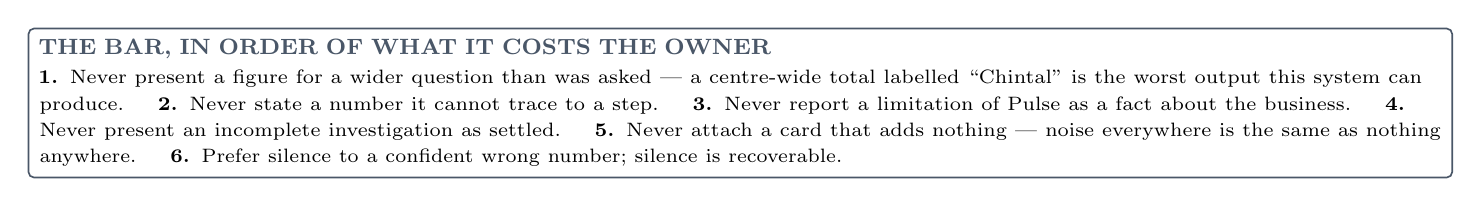
\begin{tikzpicture}
\node[box, draw=slate, fill=white, text width=178mm, align=left, font=\footnotesize]
 {\shd{THE BAR, IN ORDER OF WHAT IT COSTS THE OWNER}
  \scriptsize
  \textbf{1.} Never present a figure for a wider question than was asked --- a centre-wide total labelled
  ``Chintal'' is the worst output this system can produce. \quad
  \textbf{2.} Never state a number it cannot trace to a step. \quad
  \textbf{3.} Never report a limitation of Pulse as a fact about the business. \quad
  \textbf{4.} Never present an incomplete investigation as settled. \quad
  \textbf{5.} Never attach a card that adds nothing --- noise everywhere is the same as nothing anywhere. \quad
  \textbf{6.} Prefer silence to a confident wrong number; silence is recoverable.};
\end{tikzpicture}

\vfill
{\scriptsize\color{slate}Full detail --- the progression through all eleven architectures, every mechanism
tried and rejected with its measurement, and fifteen limitations ranked by severity --- is in
\texttt{docs/pulse-architecture.pdf} (50 pp).}

\end{document}
